\section{Esempi notevoli di anelli euclidei}

\subsection{I numeri interi: \texorpdfstring{$\ZZ$}{Z}}

Senza ombra di dubbio l'esempio più importante di anello euclideo -- nonché
l'esempio da cui si è generalizzata proprio la stessa nozione di anello
euclideo -- è l'anello dei numeri interi. \\

In questo dominio la funzione grado è canonicamente il valore assoluto:

\[g : \ZZ \setminus \{0\} \to \NN, \, k \mapsto \left|k\right|.\]

\vskip 0.1in

Infatti, chiaramente $|a| \leq |ab|\, \forall a$, $b \in \ZZ \setminus \{0\}$. Inoltre
esistono -- e sono anche unici, a meno di segno -- $q$, $r \in \ZZ \mid a = bq + r$, con $r=0 \,\lor\,
    \left|r\right| < \left|q\right|$. \\

Dal momento che così si verifica che $\ZZ$ è un anello euclideo, il \textit{Teorema
    fondamentale dell'aritmetica} è una conseguenza del
\textit{Teorema \ref{th:euclidei_ufd}}.

\subsection{I campi: \texorpdfstring{$\KK$}{K}}

Ogni campo $\KK$ è un anello euclideo, seppur banalmente. Infatti, eccetto proprio
per $0$, ogni elemento è "divisibile" per ogni altro elemento: siano $a$, $b \in \KK$,
allora $a = ab^{-1}b$. \\

Si definisce quindi la funzione grado come la funzione nulla:

\[g : \KK^* \to \NN, \, a \mapsto 0.\]

\vskip 0.1in

Chiaramente $g$ soddisfa il primo assioma della funzione grado. Inoltre,
poiché ogni elemento è "divisibile", il resto è sempre zero -- non è pertanto
necessario verificare nessun'altra proprietà.

\subsection{I polinomi di un campo: \texorpdfstring{$\KK[x]$}{K[x]}}

I polinomi di un campo $\KK$ formano un anello euclideo rilevante
nello studio dell'algebra astratta. Come suggerisce la
terminologia, la funzione grado in questo dominio coincide
proprio con il grado del polinomio, ossia si definisce come:

\[g : \KK[x] \setminus \{0\} \to \NN, \, f(x) \mapsto \deg f.\]

\vskip 0.1in

Si verifica facilmente che $g(a(x)) \leq g(a(x)b(x)) \, \forall a(x)$, $b(x) \in \KK[x] \setminus \{0\}$, mentre la divisione euclidea -- come negli interi -- ci permette
di concludere che effettivamente $\KK[x]$ soddisfa tutti gli assiomi di un anello
euclideo\footnote{Curiosamente i polinomi di $\KK[x]$ e i campi $\KK$ sono gli unici anelli euclidei in cui resti
    e quozienti sono unici, includendo la scelta di segno (vd.
    \cite{10.2307/2315810}).}.

\begin{example}
    Sia $\alpha \in \KK$ e sia $\varphi_\alpha : \KK[x] \to \KK, \, f(x) \mapsto f(\alpha)$
    la sua valutazione polinomiale in $\KK[x]$. $\varphi_\alpha$ è un omomorfismo, il cui
    nucleo è rappresentato dai polinomi in $\KK[x]$ che hanno $\alpha$ come radice. Poiché
    $\KK[x]$ è un PID, $\Ker \varphi$ deve essere monogenerato. $x-\alpha \in \Ker \varphi$
    è irriducibile, e quindi è il generatore dell'ideale. Si desume così che
    $\Ker \varphi = (x-\alpha)$.
\end{example}

\subsection{Gli interi di Gauss: \texorpdfstring{$\ZZ[i]$}{Z[i]}}

Un importante esempio di anello euclideo è il dominio degli interi di Gauss $\ZZ[i]$, definito come:

\[\ZZ[i] = \{a+bi \mid a, b \in \ZZ\}.\]

\vskip 0.1in

\begin{wrapfigure}{l}{0pt}
    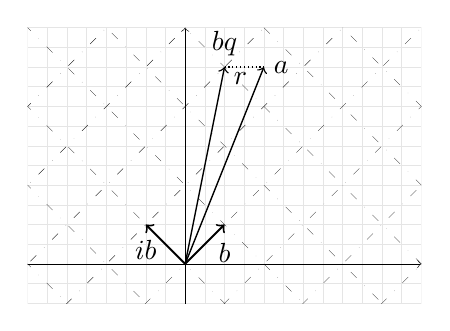
\begin{tikzpicture}
        \begin{scope}
            \clip (-2, -0.5) rectangle (3, 3);
            \draw[step=0.25cm, gray!20!white, very thin] (-7, -3) grid (7, 3);

            \foreach \x in {-4,...,4} {
                    \draw[ultra thin, loosely dashdotted] (-3 + \x, -3) -- (3 + \x, 3);
                }
            \foreach \y in {-4,...,5} {
                    \draw[ultra thin, loosely dashdotted] (-7, 7 + \y) -- (7, -7 + \y);
                }

            \draw[line width=0.7pt, ->] (0, 0) -- (0.5, 0.5) node[align=center, below=3pt]{$b$};
            \draw[line width=0.7pt, ->] (0, 0) -- (-0.5, 0.5) node[align=center, below=2pt]{$ib$};

            \draw[line width=0.5pt, ->] (0, 0) -- (0.5, 2.5) node[above=0.5pt]{$bq$};

            \draw[line width=0.5pt, ->] (0, 0) -- (1, 2.5) node[below, right]{$a$};

            \draw[densely dotted] (0.5, 2.5) -- (1, 2.5) node[below=4pt, left=2.5pt]{$r$};

            \draw[line width=0.2pt, ->] (0, -1) -- (0, 3);
            \draw[line width=0.2pt, ->] (-3, 0) -- (3, 0);

        \end{scope}
    \end{tikzpicture}
    \caption{Visualizzazione della divisione euclidea nel piano degli interi di Gauss.}
    \label{fig:z_i}
\end{wrapfigure}

La funzione grado coincide in particolare con il quadrato del modulo di un numero complesso, ossia:
\[g(z) : \ZZ[i] \setminus \{0\} \to \NN, \, a+bi \mapsto \left| a+bi \right|^2.\]

Il vantaggio di quest'ultima definizione è l'enfasi sul collegamento tra la funzione grado
di $\ZZ$ e quella di $\ZZ[i].$ Infatti, se $a \in \ZZ$, il grado di $a$ in $\ZZ$ e in $\ZZ[i]$
sono uno il quadrato dell'altro. In particolare, è possibile ridefinire il grado
di $\ZZ$ proprio in modo tale da farlo coincidere con quello di $\ZZ[i]$. \\

\begin{theorem}
    $\ZZ[i]$ è un anello euclideo.
\end{theorem}

\begin{proof}
    Si verifica la prima proprietà della funzione grado. Siano $a$, $b \in \ZZ[i] \setminus \{0\}$,
    allora $\left|a\right| \geq 1 \,\land\, \left|b\right| \geq 1$. Poiché
    $\left|ab\right| = \left|a\right|\left|b\right|$\footnote{Questa interessante proprietà del modulo è alla base dell'identità di Brahmagupta-Fibonacci: $(a^2 + b^2)(c^2 + d^2) = (ac-bd)^2 + (ad+bc)^2.$}, si verifica facilmente che
    $\left|ab\right| \geq \left|a\right|$, ossia che $g(ab) \geq g(a)$. \\

    Si verifica infine che esiste una divisione euclidea, ossia che
    $\forall a \in \ZZ[i]$, $\forall b \in \ZZ[i] \setminus \{0\}$, $\exists q$, $r \in \ZZ[i] \mid a = bq + r$ e $r=0 \,\lor\, g(r) < g(b)$.
    Come si visualizza facilmente nella \textit{Figura \ref{fig:z_i}},
    tutti i multipli di $b$ formano un piano con basi $b$ e $ib$, dove
    sicuramente esiste un certo $q$ tale che la distanza $\left|r\right| = \left|a-bq\right|$ sia minima. \\

    Se $a$ è un multiplo di $b$, vale sicuramente che $a = bq$. Altrimenti dal momento che $r$ è sicuramente inquadrato in uno dei tasselli del piano, vale
    sicuramente la seguente disuguaglianza, che lega il modulo di $r$ alla diagonale di
    ogni quadrato:

    \[\left|r\right| \leq \frac{\left|b\right|}{\sqrt{2}}.\]

    Pertanto vale la seconda e ultima proprietà della funzione grado:

    \[\left|r\right| \leq \frac{\left|b\right|}{\sqrt{2}} < \left|b\right| \implies \left|r\right|^2 < \left|b\right|^2 \implies g(r) < g(b).\]
\end{proof}

\subsection{Gli interi di Eisenstein: \texorpdfstring{$\ZZ[\omega]$}{Z[ω]}}

Sulla scia di $\ZZ[i]$ è possibile definire anche l'anello degli
interi di Eisenstein, aggiungendo a $\ZZ$ la prima radice cubica
primitiva dell'unità in senso antiorario, ossia:

\[\omega = e^{\frac{2\pi i}{3}} = -\frac{1}{2} + \frac{\sqrt{3}}{2}i.\]

In particolare, $\omega$ è una delle due radici dell'equazione
$z^2 + z + 1 = 0$, dove invece l'altra radice altro non è che
$\omega^2 = \overline{\omega}$.

\begin{wrapfigure}{l}{0pt}
    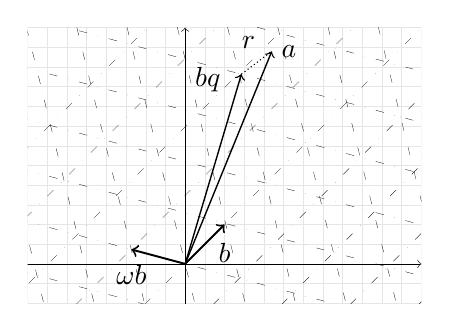
\begin{tikzpicture}
        \begin{scope}
            \clip (-2, -0.5) rectangle (3, 3);
            \draw[step=0.25cm, gray!20!white, very thin] (-7, -3) grid (7, 3);

            \foreach \x in {-4,...,4} {
                    \draw[ultra thin, loosely dashdotted] (-3 + 0.87*\x, -3) -- (3 + 0.87*\x, 3);
                }

            \foreach \y in {-4,...,5} {
                    \draw[ultra thin, loosely dashdotted] (-7, 1.8756443470179 + 0.65*\y) -- (7, -1.8756443470179 + 0.65*\y);
                }

            \foreach \x in {-4,...,5} {
                    \draw[ultra thin, loosely dashed] (-7 + 0.6289*\x, 28.5025773880714) -- (7+ 0.65*\x, -28.5025773880714);
                }

            \draw[line width=0.7pt, ->] (0, 0) -- (0.5, 0.5) node[align=center, below=3pt]{$b$};
            \draw[line width=0.7pt, ->] (0, 0) -- (-0.6830127018922, 0.1830127018922) node[align=center, below=2pt]{$\omega b$};

            \draw[line width=0.5pt, ->] (0, 0) -- (0.71494, 2.41094) node[below=2pt, left=4pt]{$bq$};

            \draw[line width=0.5pt, ->] (0, 0) -- (1.1, 2.7) node[below, right]{$a$};

            \draw[densely dotted] (0.71494, 2.41094) -- (1.1, 2.7) node[above=3pt, left=2.5pt]{$r$};

            \draw[line width=0.2pt, ->] (0, -1) -- (0, 3);
            \draw[line width=0.2pt, ->] (-3, 0) -- (3, 0);

        \end{scope}
    \end{tikzpicture}
    \caption{Visualizzazione della divisione euclidea nel piano degli interi di Eisenstein.}
    \label{fig:z_omega}
\end{wrapfigure}

\vskip 0.1in

La funzione grado in $\ZZ[\omega]$ deriva da quella di $\ZZ[i]$ e coincide ancora
con il quadrato del modulo del numero complesso. Si definisce quindi:

\[g : \ZZ[\omega] \setminus \{0\}, \, a+b\omega \mapsto \left|a+b\omega\right|^2.\]

Sviluppando il modulo è possibile ottenere una formula più concreta:

\[ \left|a+b\omega\right|^2 = \left|\left(a-\frac{b}{2}\right) + \frac{b\sqrt{3}}{2}i\right|^2 =\] \\

\[= \left(a-\frac{b}{2}\right)^2 + \frac{3b^2}{4} = a^2 - ab + b^2.\] \\

\begin{theorem}
    $\ZZ[\omega]$ è un anello euclideo.
\end{theorem}

\begin{proof}
    Sulla scia della dimostrazione presentata per $\ZZ[i]$, si verifica facilmente
    la prima proprietà della funzione grado. Siano $a$, $b \in \ZZ[\omega]$, allora
    $\left|a\right| \geq 1$ e $\left|b\right| \geq 1$. Poiché dalle proprietà
    dei numeri complessi vale ancora $\left|a\right| \left|b\right| \geq \left|a\right|$,
    la proprietà $g(ab) \geq g(a)$ è già verificata. \\

    Si verifica infine la seconda e ultima proprietà della funzione grado. Come per
    $\ZZ[i]$, i multipli di $b \in \ZZ[\omega]$ sono visualizzati su un piano che
    ha per basi $b$ e $\omega b$ (come in $\textit{Figura \ref{fig:z_omega}}$), pertanto
    esiste sicuramente un $q$ tale che la distanza $\left|a-bq\right|$ sia minima. \\

    Se $a$ è multiplo di $b$, allora chiaramente $a = bq$. Altrimenti, $a$ è certamente
    inquadrato in uno dei triangoli del piano, per cui vale la seguente disuguaglianza:

    \[\left|r\right| \leq \frac{\sqrt{3}}{2} \left|b\right|.\]

    Dunque la tesi è verificata:

    \[\left|r\right| \leq \frac{\sqrt{3}}{2} \left|b\right| < \left|b\right| \implies \left|r\right|^2 < \left|b\right|^2 \implies g(r) < g(b). \]
\end{proof}
